\documentclass{./SAS-class-skygen}
    
    \newcommand{\hwnum}{Сборная Москвы}
	\newcommand{\subject}{№11}
	\newcommand{\skykey}{41.96 00:08}
    
    \begin{document}
    
    
    
	\begin{center}
		\large\textbf{Ежедневный скайчарт №11}
	\end{center}

	\begin{enumerate}
		\item Обозначьте точку зенита символом \boldsans{Z} и стороны света как \boldsans{N}, \boldsans{E}, \boldsans{S}, \boldsans{W}.
		\item Обозначьте полюс мира символом \boldsans{P}.
		\item Обозначьте точку весны символом \Aries. Или же точку осени символом \Libra.
		\item Проведите большие круги небесного экватора и эклиптики.
		\item Рассчитайте звёздное время скайчарта: \rule{2cm}{0.4pt}
		\item Определите широту места съёмки: \rule{2cm}{0.4pt}
		\item Проведите контуры всех видимых созвездий, а также напишите их обозначения по Байеру.
		\item Отметьте на скайчарте небесные объекты, приведённые в таблице ниже.
	\end{enumerate}
	
    \vspace{0.5cm}

    \begin{table}[h!]
    \centering
    \begin{tabular}{ccc}
    \multicolumn{3}{c}{\textbf{Звёзды}} \\ Окаб & Беллатрикс & Каф \\
Альдерамин & Бетельгейзе & Альферац \\
Эниф & Мирах & Денеб Альгеди \\

\end{tabular}
    \hfill
    \begin{tabular}{ccc}
    \multicolumn{3}{c}{\textbf{Объекты Мессье}} \\ M13 & M103 & M73 \\
M51 & M2 & M35 \\
M37 & M40 & M77 \\

\end{tabular}
    \end{table}
	
	\vspace{0.5cm}
    \begin{center}
    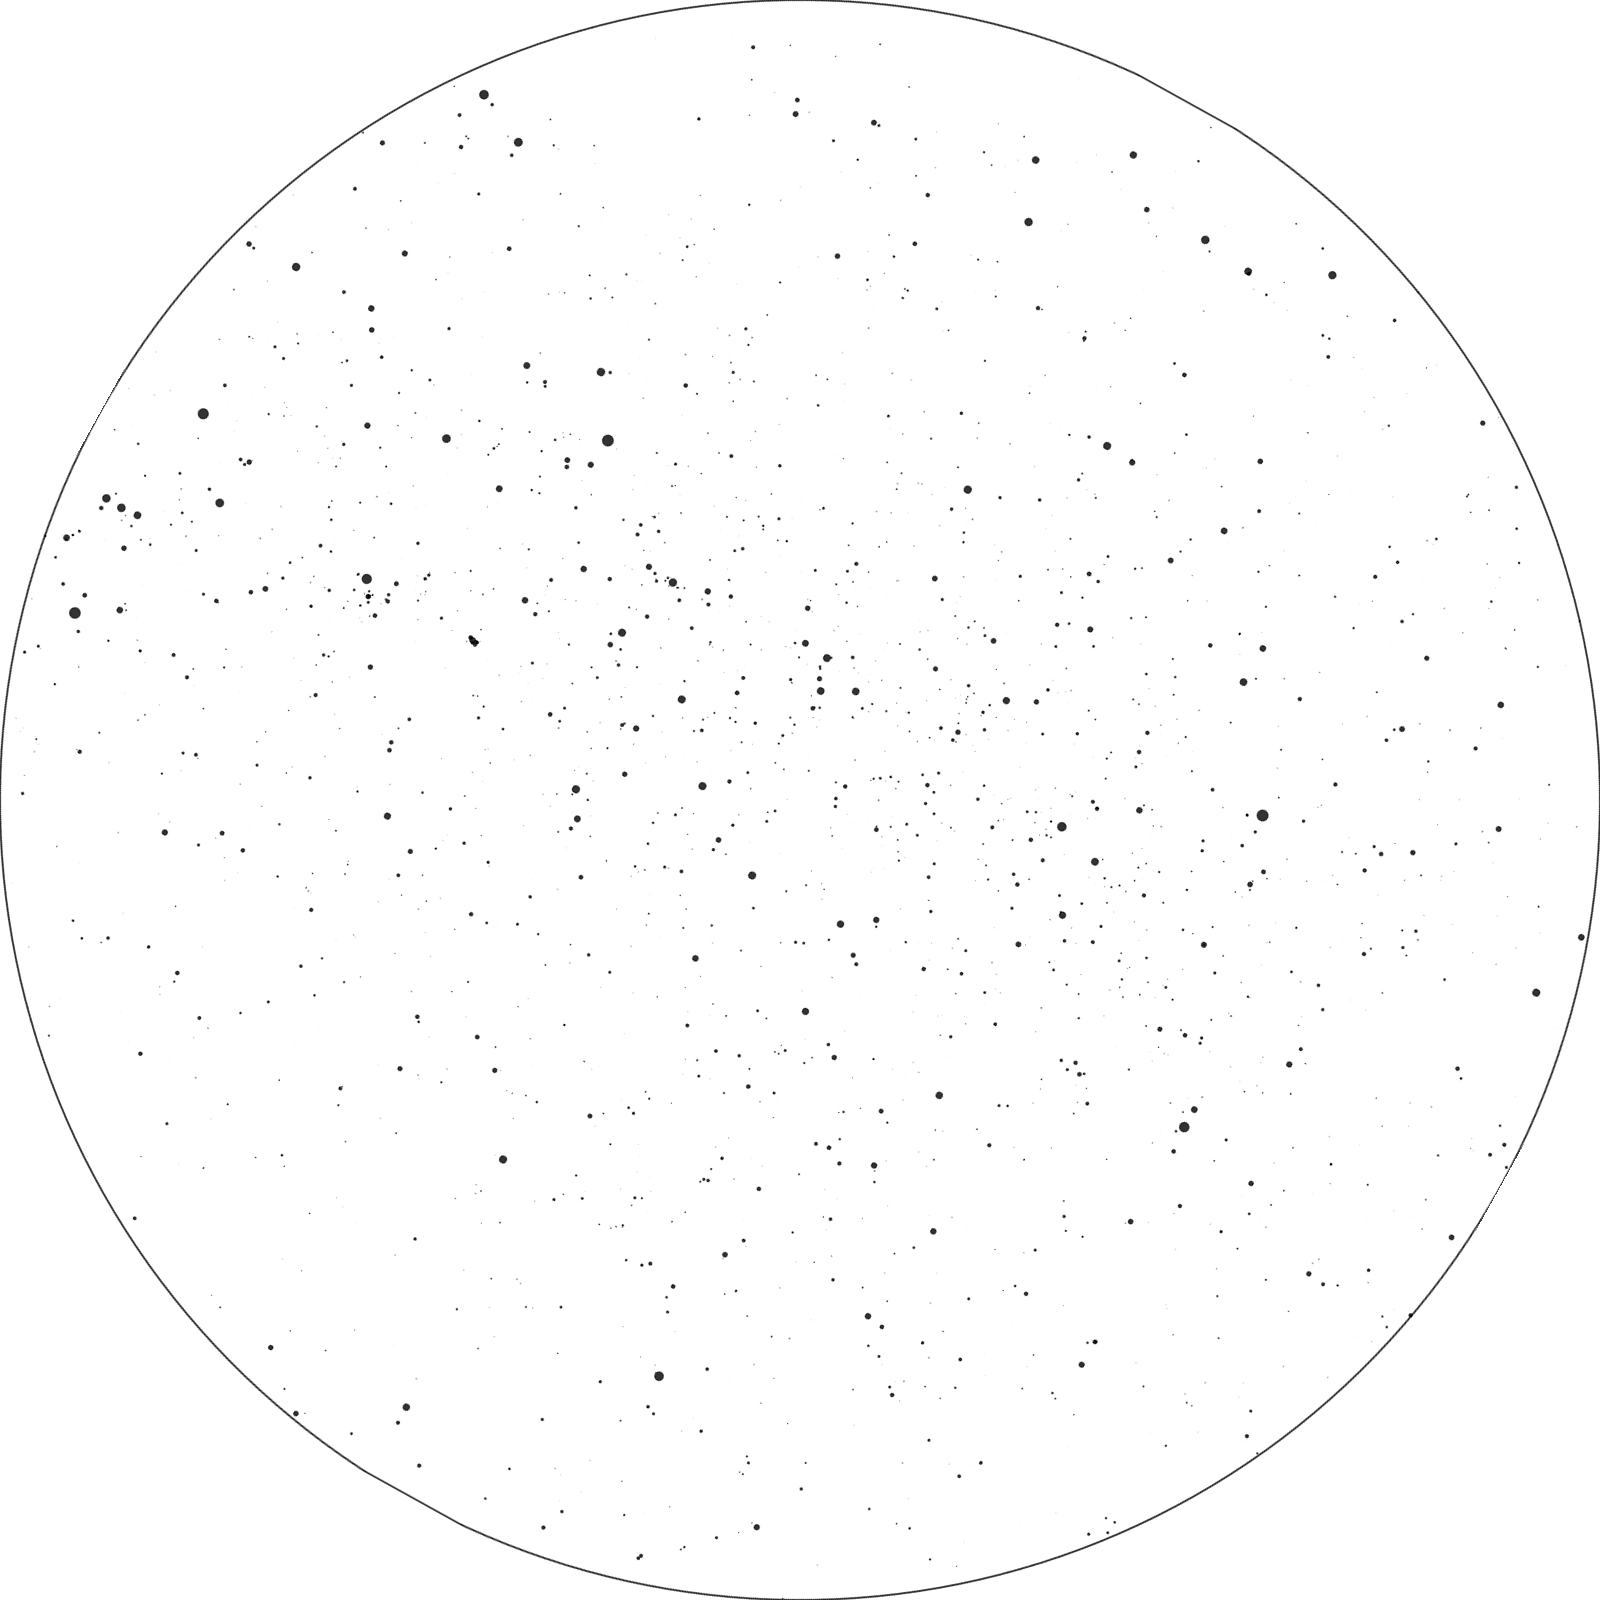
\includegraphics[width=\textwidth]{./pics/skychart11.png}
    \end{center}
    
    \end{document}
    